\documentclass[a4paper,12pt]{article}
\usepackage{newlistok}
\usepackage{tikz}\usetikzlibrary{calc,through,intersections,backgrounds,arrows,decorations.pathreplacing}
\usepackage{tkz-euclide}

\УвеличитьВысоту{1.5cm}
\УвеличитьШирину{1.5cm}


\begin{document}

Ломанные в абсолютных координатах, жирность, цвет, параллельный перенос\\
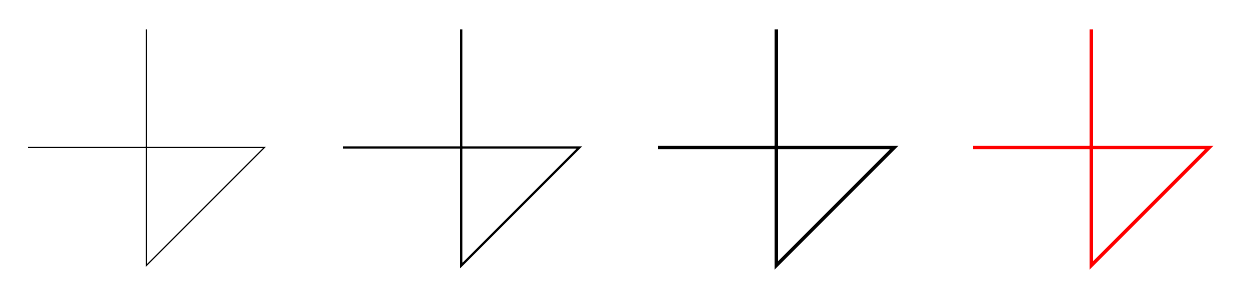
\begin{tikzpicture}
  \draw (-1.5,0) -- (1.5,0) -- (0,-1.5) -- (0,1.5);
  \draw[xshift=4cm, thick] (-1.5,0) -- (1.5,0) -- (0,-1.5) -- (0,1.5);
  \draw[xshift=8cm, very thick] (-1.5,0) -- (1.5,0) -- (0,-1.5) -- (0,1.5);
  \draw[xshift=12cm, very thick, color=red] (-1.5,0) -- (1.5,0) -- (0,-1.5) -- (0,1.5);
\end{tikzpicture}
\begin{verbatim}
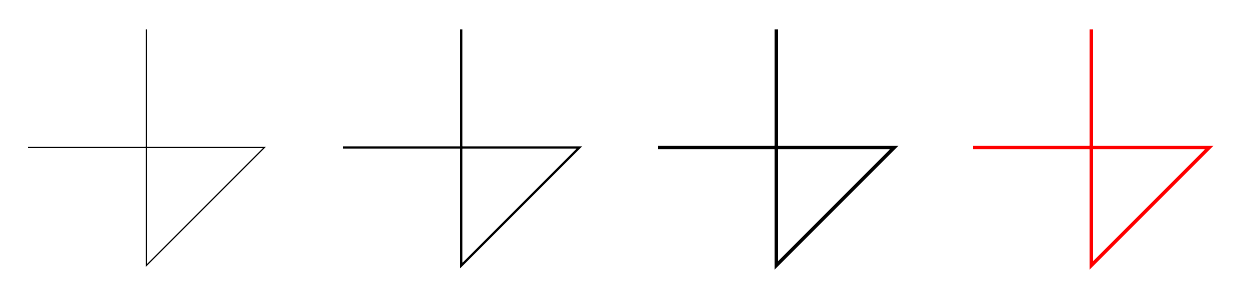
\begin{tikzpicture}
  \draw (-1.5,0) -- (1.5,0) -- (0,-1.5) -- (0,1.5);
  \draw[xshift=4cm, thick] (-1.5,0) -- (1.5,0) -- (0,-1.5) -- (0,1.5);
  \draw[xshift=8cm, very thick] (-1.5,0) -- (1.5,0) -- (0,-1.5) -- (0,1.5);
  \draw[xshift=12cm, very thick, color=red] (-1.5,0) -- (1.5,0) -- (0,-1.5) -- (0,1.5);
\end{tikzpicture}
\end{verbatim}



Вместо абсолютных координат можно указывать абсолютные полярные в формате (угол:радиус)\\
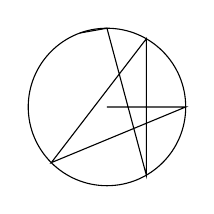
\begin{tikzpicture}
  \draw (0,0) circle (1);
  \draw (0,0) -- (0:1) -- (-135:1) -- (60:1) -- (-60:1) -- (90:1) -- (110:1) ;
\end{tikzpicture}
\begin{verbatim}
  \draw (0,0) circle (1);
  \draw (0,0) -- (0:1) -- (-135:1) -- (60:1) -- (-60:1) -- (90:1) -- (110:1) ;
\end{verbatim}



Относительные координаты
\begin{tikzpicture}
  \draw[green, very thick]  (0,0) -- (1,0) -- (1,1) -- (2,1); % Абсолютные координаты
  \draw[blue, dashed ]  (2,0) -- +(1,0) -- +(1,1) -- +(2,1); %
  % (3,0) устанавливает текущую позицию,  +(1,0) --- свдиг от текущей позиции
  \draw[red] (4,0) -- ++(1,0) --  ++(1,1) --  ++(-30:1);
  % (5,0) устанавливает текущую позицию,  ++(1,0) --- свдиг от текущей позиции, затем установка новой текущей позиции
\end{tikzpicture}
\begin{verbatim}
  \draw[green, very thick]  (0,0) -- (1,0) -- (1,1) -- (2,1); % Абсолютные координаты
  \draw[blue, dashed ]  (2,0) -- +(1,0) -- +(1,1) -- +(2,1); %
  % (3,0) устанавливает текущую позицию,  +(1,0) --- свдиг от текущей позиции
  \draw[red] (4,0) -- ++(1,0) --  ++(1,1) --  ++(-30:1);
  % (5,0) устанавливает текущую позицию,
  % ++(1,0) --- сдвиг от текущей позиции, затем установка новой текущей позиции
\end{verbatim}











Окружность, эллипс, куски дуг, прямоугольник\\
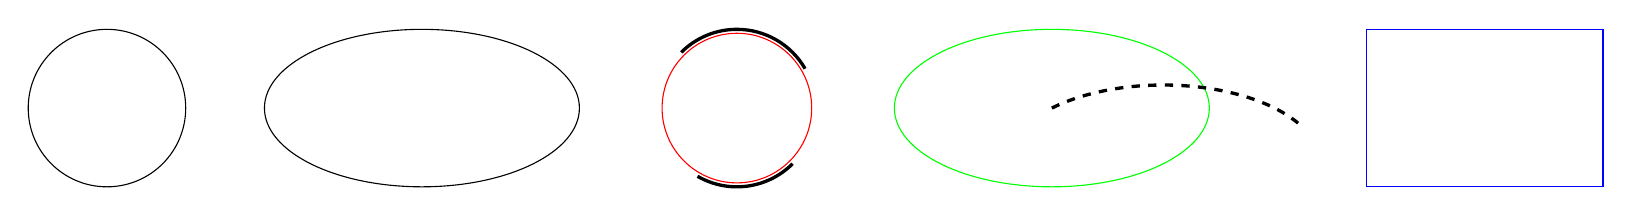
\begin{tikzpicture}
  \draw (0,0) circle (1);
  \draw[xshift=4cm] (0,0) ellipse (2 and 1);

  \draw[xshift=8cm, red, thin] (0,0) circle (.95);
  \draw[xshift=8cm, very thick] (30:1) arc (30:135:1)
                                (-45:1) arc (-45:-120:1);

  \draw[xshift=12cm, green] (0,0) ellipse (2 and 1);
  \draw[xshift=12cm, very thick, dashed] (0,0) arc (135:30:2 and 1);
  \draw[xshift=16cm, blue] (0,-1) rectangle +(3,2);
\end{tikzpicture}
\begin{verbatim}
  \draw (0,0) circle (1);
  \draw[xshift=4cm] (0,0) ellipse (2 and 1);

  \draw[xshift=8cm, red, thin] (0,0) circle (.95);
  \draw[xshift=8cm, very thick] (30:1) arc (30:135:1)
                                (-45:1) arc (-45:-120:1);

  \draw[xshift=12cm, green] (0,0) ellipse (2 and 1);
  \draw[xshift=12cm, very thick, dashed] (0,0) arc (135:30:2 and 1);
  \draw[xshift=16cm, blue] (0,-1) rectangle +(3,2);
\end{verbatim}


\newpage
Заливка с контуром и без
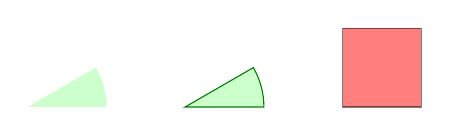
\begin{tikzpicture}
  \fill[fill=green!20] (0,0) -- (1,0) arc (0:30:1) -- cycle;
  \filldraw[fill=green!20,draw=green!50!black] (2,0) -- (3,0) arc (0:30:1) -- cycle;
  \draw[fill=red, opacity=0.5] (4,0) -- +(1,0) -- +(1,1) -- +(0,1) -- cycle;  % прозрачность
\end{tikzpicture}
\begin{verbatim}
  \fill[fill=green!20] (0,0) -- (1,0) arc (0:30:1) -- cycle;
  \filldraw[fill=green!20,draw=green!50!black] (2,0) -- (3,0) arc (0:30:1) -- cycle;
  \draw[fill=red, opacity=0.5] (4,0) -- +(1,0) -- +(1,1) -- +(0,1) -- cycle;  % прозрачность
\end{verbatim}


Координатные сетки
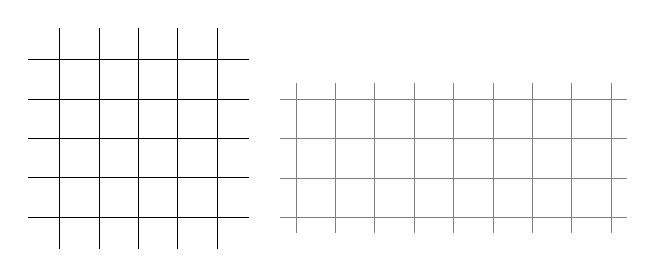
\begin{tikzpicture}
  \draw[step=.5] (-1.4,-1.4) grid (1.4,1.4);
  \draw[step=1,gray,very thin, xshift=2cm, yshift=-1cm, scale=0.5] (-.4,-.4) grid (8.4,3.4);
\end{tikzpicture}
\begin{verbatim}
  \draw[step=.5] (-1.4,-1.4) grid (1.4,1.4);
  \draw[step=1,gray,very thin, xshift=2cm, yshift=-1cm, scale=0.5] (-.4,-.4) grid (8.4,3.4);
\end{verbatim}



Кривые
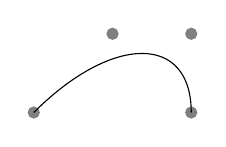
\begin{tikzpicture}
\filldraw [gray] (0,0) circle (2pt)
(1,1) circle (2pt)
(2,1) circle (2pt)
(2,0) circle (2pt);
\draw (0,0) .. controls (1,1) and (2,1) .. (2,0);
\end{tikzpicture}
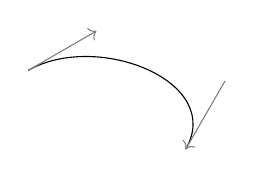
\begin{tikzpicture}
    \draw (2,0) .. controls +(30:1cm) and +(60:1cm) .. (4,-1);
    \draw[gray,->] (2,0) -- +(30:1cm);
    \draw[gray,<-] (4,-1) -- +(60:1cm);
\end{tikzpicture}
\begin{verbatim}
    \filldraw [gray] (0,0) circle (2pt)
                     (1,1) circle (2pt)  % сначала стремимся сюда
                     (2,1) circle (2pt)  % затем сюда
                     (2,0) circle (2pt);
    \draw (0,0) .. controls (1,1) and (2,1) .. (2,0);

    \draw (1,0) .. controls +(30:1cm) and +(60:1cm) .. (3,-1); % Относительные координаты
    \draw[gray,->] (1,0) -- +(30:1cm);
    \draw[gray,<-] (3,-1) -- +(60:1cm);
\end{verbatim}

Обрезка снаружи от области
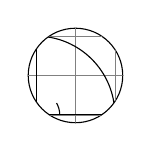
\begin{tikzpicture}[scale=1]
    \clip[draw] (0.5,0.5) circle (.6cm);
    \draw[step=.5cm,gray,very thin] (-1.4,-1.4) grid (1.4,1.4);
    \draw (-1.5,0) -- (1.5,0);
    \draw (0,-1.5) -- (0,1.5);
    \draw (0,0) circle (1cm);
    \draw (3mm,0mm) arc (0:30:3mm);
\end{tikzpicture}
\begin{verbatim}
    \clip[draw] (0.5,0.5) circle (.6cm);
    \draw[step=.5cm,gray,very thin] (-1.4,-1.4) grid (1.4,1.4);
    \draw (-1.5,0) -- (1.5,0);
    \draw (0,-1.5) -- (0,1.5);
    \draw (0,0) circle (1cm);
    \draw (3mm,0mm) arc (0:30:3mm);
\end{verbatim}

Стрелки
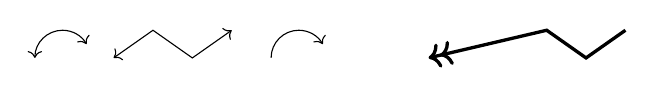
\begin{tikzpicture}
    \draw [<->] (0,0) arc (180:30:10pt);
    \draw [<->] (1,0) -- (1.5cm,10pt) -- (2cm,0pt) -- (2.5cm,10pt);
    \draw [->] (3,0) arc (180:30:10pt);
    \draw [<<-,very thick] (5,0) -- +(1.5cm,10pt) -- +(2cm,0pt) -- +(2.5cm,10pt);
\end{tikzpicture}
\begin{verbatim}
    \draw [<->] (0,0) arc (180:30:10pt);
    \draw [<->] (1,0) -- (1.5cm,10pt) -- (2cm,0pt) -- (2.5cm,10pt);
    \draw [->] (3,0) arc (180:30:10pt);
    \draw [<<-,very thick] (5,0) -- +(1.5cm,10pt) -- +(2cm,0pt) -- +(2.5cm,10pt);
\end{verbatim}





Подписи
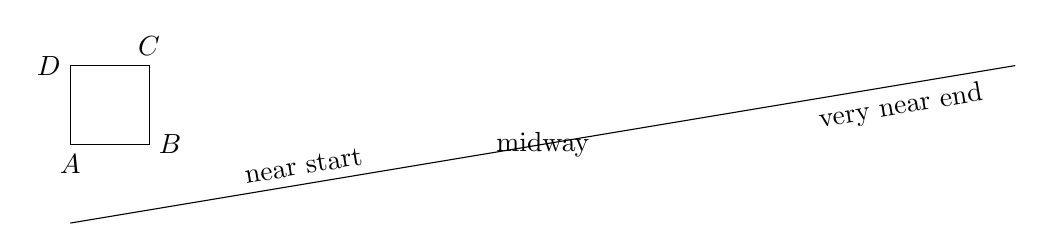
\begin{tikzpicture}
  \draw (0,0) node[below] {$A$} -- (1,0) node[right] {$B$} -- (1,1) node[above] {$C$} -- (0,1) node[left] {$D$} -- cycle;
  \draw (0, -1) -- node[near start, sloped, above] {near start}
                   node[midway] {midway}
                   node[very near end, sloped, below] {very near end} (12, 1);
\end{tikzpicture}
\begin{verbatim}
  \draw (0,0) node[below] {$A$} -- (1,0) node[right] {$B$} -- (1,1) node[above] {$C$} -- (0,1) node[left] {$D$} -- cycle;
  \draw (0, -1) -- node[near start, sloped, above] {near start}
                   node[midway] {midway}
                   node[very near end, sloped, below] {very near end} (12, 1);
\end{verbatim}





\newpage
Циклы
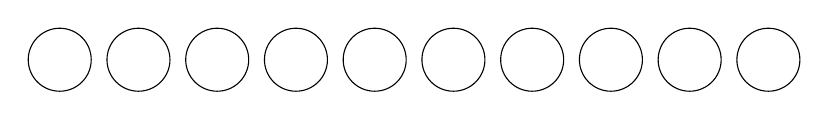
\begin{tikzpicture}
    \foreach \x in {1,...,10}
        \draw (\x,0) circle (0.4cm);
\end{tikzpicture}
\begin{tikzpicture}
    \foreach \x in {-1,-0.5,...,1}
        \draw (\x cm,-2pt) -- (\x cm,2pt);
\end{tikzpicture}\\
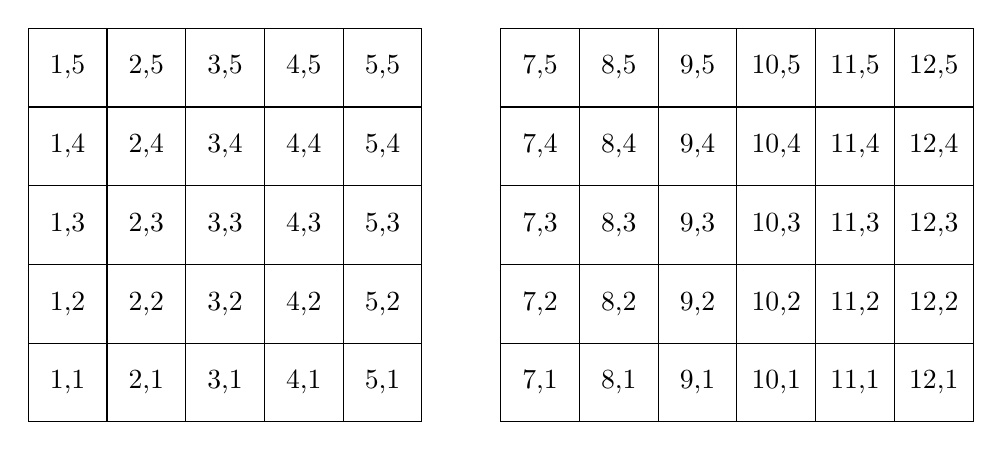
\begin{tikzpicture}
\foreach \x in {1,2,...,5,7,8,...,12}
    \foreach \y in {1,...,5}
    {
        \draw (\x,\y) +(-.5,-.5) rectangle ++(.5,.5);
        \draw (\x,\y) node{\x,\y};
    }
\end{tikzpicture}
\begin{verbatim}
    \foreach \x in {1,...,10}
        \draw (\x,0) circle (0.4cm);
    \foreach \x in {-1,-0.5,...,1}
        \draw (\x cm,-2pt) -- (\x cm,2pt);
    \foreach \x in {1,2,...,5,7,8,...,12}
        \foreach \y in {1,...,5}
        {
            \draw (\x,\y) +(-.5,-.5) rectangle ++(.5,.5);
            \draw (\x,\y) node{\x,\y};
        }
\end{verbatim}




Циклы с парами координат
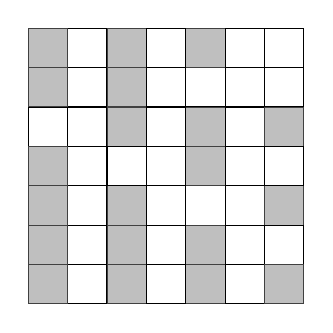
\begin{tikzpicture}[scale=.5]
  \draw[step=1] (0,0) grid (7,7);
  \foreach \x/\y/\h in {0/0/4, 0/5/2, 2/0/3, 2/4/3, 4/0/2, 4/3/2, 4/6/1, 6/0/1, 6/2/1, 6/4/1}
    \fill[gray,opacity=0.5] (\x,\y) rectangle +(1,\h);
\end{tikzpicture}
\begin{verbatim}
  \draw[step=1] (0,0) grid (7,7);
  \foreach \x/\y/\h in {0/0/4, 0/5/2, 2/0/3, 2/4/3, 4/0/2, 4/3/2, 4/6/1, 6/0/1, 6/2/1, 6/4/1}
    \fill[gray,opacity=0.5] (\x,\y) rectangle +(1,\h);
\end{verbatim}






Обозначаем координаты точек и пути
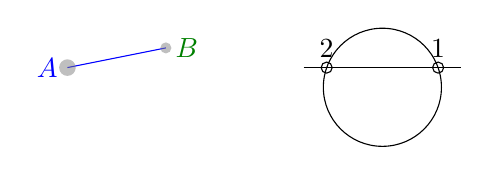
\begin{tikzpicture}
    \coordinate [label=left:\textcolor{blue}{$A$}] (A) at (0,0);
    \coordinate [label=right:\textcolor{green!50!black}{$B$}] (B) at (1.25,0.25);
    \draw[blue] (A) -- (B);
    \fill[color=gray,opacity=0.5] (A) circle (3pt) (B) circle (2pt);
    \draw[name path=myline] (3, 0) -- (5, 0);  % Рисуем и обозначаем
    \draw[name path=mycircle] (4,-0.25) circle (.75); % Только обозначаем
    \draw [name intersections={of=myline and mycircle}]
        (intersection-1) circle (2pt) node[above] {1}
        (intersection-2) circle (2pt) node[above] {2};
\end{tikzpicture}
\begin{verbatim}
    \coordinate [label=left:\textcolor{blue}{$A$}] (A) at (0,0);
    \coordinate [label=right:\textcolor{green!50!black}{$B$}] (B) at (1.25,0.25);
    \draw[blue] (A) -- (B);
    \fill[color=gray,opacity=0.5] (A) circle (3pt) (B) circle (2pt);
    \draw[name path=myline] (3, 0) -- (5, 0);  % Рисуем и обозначаем
    \draw[name path=mycircle] (4,-0.25) circle (.75); % Только обозначаем
    \draw [name intersections={of=myline and mycircle}]
        (intersection-1) circle (2pt) node[above] {1}
        (intersection-2) circle (2pt) node[above] {2};
\end{verbatim}




\newpage

Проекция точки на отрезок
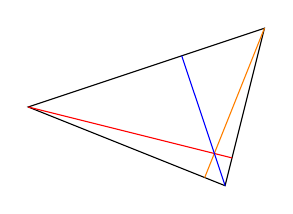
\begin{tikzpicture}
    \coordinate (a) at (0,1);
    \coordinate (b) at (3,2);
    \coordinate (c) at (2.5,0);
    \draw (a) -- (b) -- (c) -- cycle;
    \draw[red] (a) -- ($(b)!(a)!(c)$);
    \draw[orange] (b) -- ($(a)!(b)!(c)$);
    \draw[blue] (c) -- ($(a)!(c)!(b)$);
\end{tikzpicture}
\begin{verbatim}
    \coordinate (a) at (0,1);
    \coordinate (b) at (3,2);
    \coordinate (c) at (2.5,0);
    \draw (a) -- (b) -- (c) -- cycle;
    \draw[red] (a) -- ($(b)!(a)!(c)$);
    \draw[orange] (b) -- ($(a)!(b)!(c)$);
    \draw[blue] (c) -- ($(a)!(c)!(b)$);
\end{verbatim}



Делим отрезов в нужном отношении
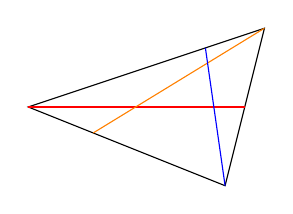
\begin{tikzpicture}
    \coordinate (a) at (0,1);
    \coordinate (b) at (3,2);
    \coordinate (c) at (2.5,0);
    \draw (a) -- (b) -- (c) -- cycle;
    \draw[red] (a) -- ($(b)!0.5!(c)$);
    \draw[orange] (b) -- ($(a)!0.33!(c)$);
    \draw[blue] (c) -- ($(a)!0.75!(b)$);
\end{tikzpicture}
\begin{verbatim}
    \coordinate (a) at (0,1);
    \coordinate (b) at (3,2);
    \coordinate (c) at (2.5,0);
    \draw (a) -- (b) -- (c) -- cycle;
    \draw[red] (a) -- ($(b)!0.5!(c)$);
    \draw[orange] (b) -- ($(a)!0.33!(c)$);
    \draw[blue] (c) -- ($(a)!0.75!(b)$);
\end{verbatim}





Пересекаем окружности, проводим окружность с центром в данной через другую точку
\begin{tikzpicture}[scale=1.8]
    \path [use as bounding box] (0,-1) rectangle (1.8,1);
    \coordinate [label=above:{$A$}] (A) at (60:1);
    \coordinate [label=below:{$B$}] (B) at (-60:1);
    \coordinate                     (C) at (0,0);
    \coordinate                     (D) at (1,0);
    \node [name path=circ1,circle through=(B)] at (A) {};
    \node [name path=circ2,circle through=(D)] at (B) {};
    \path [name intersections={of=circ1 and circ2}];
    \coordinate [label=right:{$B'$}] (E) at (intersection-2);
    \path [name path=circ1] (A) circle (1);
    \path [name path=circ2] (E) circle (1);
    \path [name intersections={of=circ1 and circ2}];
    \coordinate (F) at (intersection-1);
    \coordinate (G) at (intersection-2);
    \draw[thick, color=green] (A) -- (C) -- (B) -- (D) -- (A) (C) -- (D);
    \draw (A) -- (F) -- (E) -- (G) -- (A) (F) -- (G) (B) -- node[sloped, above] {\footnotesize 100\,м} (E);
    \foreach \pt in {(A), (B), (C), (D), (E), (F), (G)}
        \fill[black,opacity=.8] \pt circle (1pt);
    \draw[very thin, dashed] (B) ++(-10:1) arc (-10:45:1);
    \draw[very thin, dashed] (B) let \p1 = ($(B)-(A)$) in arc (-90:-45:{veclen(\x1,\y1)});
    \draw[thick, color=red, dashed, ->] (B) let \p1 = ($(B)-(A)$) in arc (-90:-60:{veclen(\x1,\y1)});
\end{tikzpicture}
{\footnotesize
\begin{verbatim}
    \path [use as bounding box] (0,-1) rectangle (1.8,1);
    \coordinate [label=above:{$A$}] (A) at (60:1);
    \coordinate [label=below:{$B$}] (B) at (-60:1);
    \coordinate                     (C) at (0,0);
    \coordinate                     (D) at (1,0);
    \node [name path=circ1,circle through=(B)] at (A) {};
    \node [name path=circ2,circle through=(D)] at (B) {};
    \path [name intersections={of=circ1 and circ2}];
    \coordinate [label=right:{$B'$}] (E) at (intersection-2);
    \path [name path=circ1] (A) circle (1);
    \path [name path=circ2] (E) circle (1);
    \path [name intersections={of=circ1 and circ2}];
    \coordinate (F) at (intersection-1);
    \coordinate (G) at (intersection-2);
    \draw[thick, color=green] (A) -- (C) -- (B) -- (D) -- (A) (C) -- (D);
    \draw (A) -- (F) -- (E) -- (G) -- (A) (F) -- (G) (B) -- node[sloped, above] {\footnotesize 100\,м} (E);
    \foreach \pt in {(A), (B), (C), (D), (E), (F), (G)}
        \fill[black,opacity=.8] \pt circle (1pt);
    \draw[very thin, dashed] (B) ++(-10:1) arc (-10:45:1);
    \draw[very thin, dashed] (B) let \p1 = ($(B)-(A)$) in arc (-90:-45:{veclen(\x1,\y1)});
    \draw[thick, color=red, dashed, ->] (B) let \p1 = ($(B)-(A)$) in arc (-90:-60:{veclen(\x1,\y1)});
\end{verbatim}

}



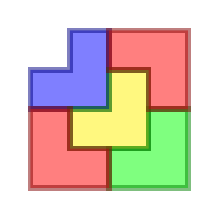
\begin{tikzpicture}[scale=0.5,
sg/.style={fill=green, draw=green!50!black, opacity=0.5, line width=2pt},
sr/.style={fill=red, draw=red!50!black, opacity=0.5, thick, line width=2pt},
sb/.style={fill=blue, draw=blue!50!black, opacity=0.5, thick, line width=2pt},
sy/.style={fill=yellow, draw=green!50!black, opacity=0.5, thick, line width=2pt},
]
\filldraw[sg] (2,0)--+(0,1)--+(1,1)--+(1,2)--+(2,2)--+(2,0)--cycle;
\filldraw[sb] (0,2)--+(0,1)--+(1,1)--+(1,2)--+(2,2)--+(2,0)--cycle;
\filldraw[sy] (1,1)--+(0,1)--+(1,1)--+(1,2)--+(2,2)--+(2,0)--cycle;
\filldraw[sr,rotate=90] (2,-4)--+(0,1)--+(1,1)--+(1,2)--+(2,2)--+(2,0)--cycle;
\filldraw[sr,rotate=-90] (-2,0)--+(0,1)--+(1,1)--+(1,2)--+(2,2)--+(2,0)--cycle;
\end{tikzpicture}



\begin{tikzpicture}[scale=1.5]
\coordinate [label=above:{$X$}] (X) at (0.5,1.2);
\coordinate [label=left:{$А$}] (A) at (0,0);
\coordinate [label=right:{$Б$}] (B) at (2,0);
\draw[thin, name path=ort] (1,2) -- (1, -.5) node[below] {\textbf{а)}};
\fill[yellow,opacity=0.2] (-0.5,-0.5) rectangle (1, 2);
\draw[thick, red, name path=A--X] (A)--(X);
\draw[thick, green, name path=A--X] (B)--(X);
\path [name intersections={of=A--X and ort,by=E}];
\draw (E) node[above right] {$M$};
\draw[thick, green] (A)--(E);
\draw(A)--(B);
\coordinate [label=below right:{$H$}] (M) at ($(A)!0.5!(B)$);
\tkzMarkSegment[color=black,pos=.5,mark=|](A,M)\tkzMarkSegment[color=black,pos=.5,mark=|](B,M)
\tkzMarkSegment[color=green,pos=.5,mark=||](A,E)\tkzMarkSegment[color=green,pos=.5,mark=||](B,E)
\foreach \pt in {(X), (A), (B), (E), (M)} \fill[black] \pt circle (1pt);
\end{tikzpicture}
\begin{tikzpicture}[scale=3]
\draw[very thick, name path=road] (0,0) -- (1.2,0);
\draw[thin, dashed, name path=ort] (1,1) -- (1, -.5);
\fill[yellow,opacity=0.2] (0.0,-0.2) rectangle (1, 1);
\path [name intersections={of=road and ort,by=B}];
\draw (B) node[below right] {$Б$};
\coordinate [label=above:{$A$}] (A) at (0.3,0.5);
\draw[green] (A)--(B);
\coordinate [label=above:{$H$}] (M) at ($(A)!0.5!(B)$);
\draw[thin, name path=bisect] (M) -- ($(M)!1.3!90:(A)$);
\path [name intersections={of=road and bisect,by=R}];
\draw[line width=4pt, red, opacity=0.5] (0,0) -- (R);
\draw (A)--(R);
\draw (R) node[below right] {$M$};
\tkzMarkSegment[color=blue,pos=.5,mark=|](A,R)
\tkzMarkSegment[color=blue,pos=.5,mark=|](R,B)
\tkzMarkSegment[color=green,pos=.5,mark=||](A,M)
\tkzMarkSegment[color=green,pos=.5,mark=||](M,B)
\foreach \pt in {(M), (A), (B), (R)} \fill[black] \pt circle (.5pt);
\draw (.6,-.2) node[below] {\textbf{б)}, \textbf{в)}};
\end{tikzpicture}


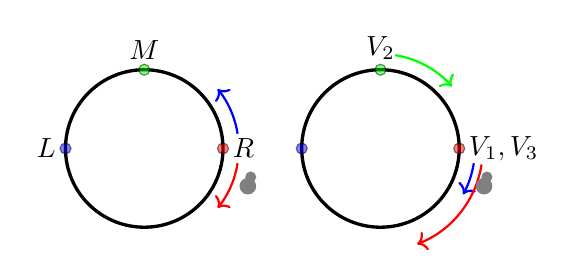
\begin{tikzpicture}
\draw[very thick] (0,0) circle (1);
\filldraw[fill=green,opacity=0.5] (90:1) circle (2pt)  ;
\filldraw[fill=red,opacity=0.5] (0:1) circle (2pt) ;
\filldraw[fill=blue,opacity=0.5] (180:1) circle (2pt) ;
\draw (90:1) node[above] {$M$}  (0:1) node[right] {$R$}  (180:1) node[left] {$L$};
\draw[->,color=red,thick] (-9:1.2) arc (-9:-39:1.2);
\draw[->,color=blue,thick] (9:1.2) arc (9:39:1.2);
\fill[color=gray] (-15:1.4) circle (2pt);
\fill[color=gray] (-20:1.4) circle (3pt);
\begin{scope}[xshift=3cm]
\draw[very thick] (0,0) circle (1);
\filldraw[fill=green,opacity=0.5] (90:1) circle (2pt);
\filldraw[fill=red,opacity=0.5] (0:1) circle (2pt);
\filldraw[fill=blue,opacity=0.5] (180:1) circle (2pt) ;
\draw (90:1) node[above] {$V_2$}  (0:1) node[right] {$V_1,V_3$};
\draw[->,color=green,thick] (81:1.2) arc (81:41:1.2);
\draw[->,color=blue,thick] (-9:1.2) arc (-9:-29:1.2);
\draw[->,color=red,thick] (-9:1.3) arc (-9:-69:1.3);
\fill[color=gray] (-15:1.4) circle (2pt);
\fill[color=gray] (-20:1.4) circle (3pt);
\end{scope}
\end{tikzpicture}

\begin{tikzpicture}
    \newdimen\R\R=1cm
    \begin{scope}[xshift=0\R]
        \draw (0:1\R) \foreach \x in {90,180,...,359} {
                -- (\x:1\R)
            } -- cycle (90:1\R) node[above] {\textbf{а})} ;
        \foreach \x in {90,180,...,360} {
            \fill[black] (\x:1\R) circle (1.5pt);
            }
    \end{scope}
    \begin{scope}[xshift=2.5\R]
        \draw (0:1\R) \foreach \x in {72,144,...,359} {
                -- (\x:1\R)
            } -- cycle (90:1\R) node[above] {\textbf{б})} ;
        \foreach \x in {72,144,...,360} {
            \fill[black] (\x:1\R) circle (1.5pt);
            }
    \end{scope}

    \begin{scope}[xshift=5\R]
        \draw (0:1\R) \foreach \x in {72,144,...,359} {
                -- (\x:1\R)
            } -- cycle (90:1\R) node[above] {\textbf{в})} ;
        \foreach \x in {72,144,...,360} {
            \fill[black] (\x:1\R) circle (1.5pt);
            }
        \fill[black] (0,0) circle (1.5pt);
    \end{scope}
\end{tikzpicture}

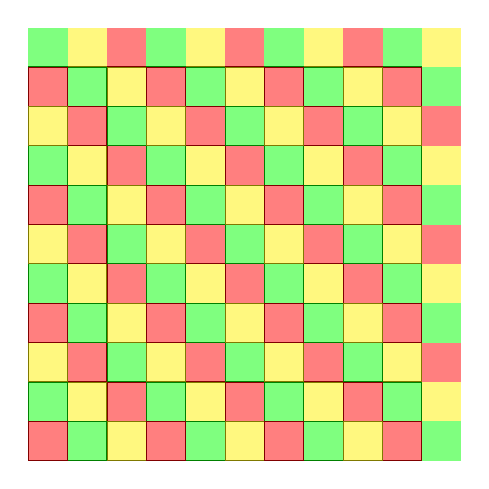
\begin{tikzpicture}[scale=0.5]
  \draw (0,0) grid(10,10);
  \foreach \x in {0,...,10} \foreach \y in {0,...,10}
{
  \pgfmathparse{int(mod(\x+\y,3))}
  \let\r\pgfmathresult
  \ifnum\r=0
  \path[fill=red, opacity = 0.5] (\x,\y) rectangle +(1,1);
  \fi
  \ifnum\r=1
  \path[fill=green, opacity = 0.5] (\x,\y) rectangle +(1,1);
  \fi
  \ifnum\r=2
  \path[fill=yellow, opacity = 0.5] (\x,\y) rectangle +(1,1);
  \fi
}
\end{tikzpicture}


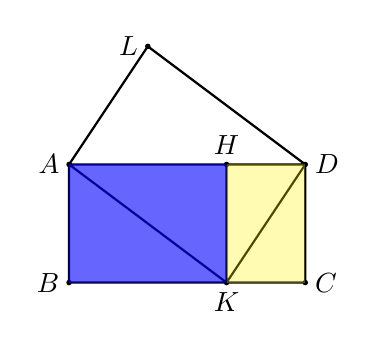
\begin{tikzpicture}[scale=0.5]
    \coordinate [label=left:{$A$}] (A) at (0,3);
    \coordinate [label=left:{$B$}] (B) at (0,0);
    \coordinate [label=right:{$C$}] (C) at (6,0);
    \coordinate [label=right:{$D$}] (D) at (6,3);
    \coordinate [label=below:{$K$}] (K) at (4,0);
    \coordinate [label=left:{$L$}] (L) at (2,6);
    \coordinate [label=above:{$H$}] (H) at (4,3);
    \foreach \pt in {(A), (B), (C), (D), (K), (L), (H)} \fill[black] \pt circle (2pt);
    \draw[thick] (A)--(B)--(C)--(D)--cycle (L)--(A)--(K)--(D)--cycle (K)--(H);
    \fill[blue, opacity=0.6] (A)--(H)--(K)--(B)--cycle;
    \fill[yellow, opacity=.3] (D)--(H)--(K)--(C)--cycle;
\end{tikzpicture}

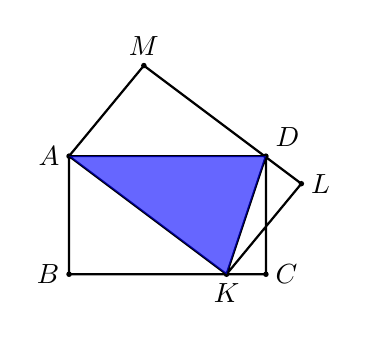
\begin{tikzpicture}[scale=0.5]
    \coordinate [label=left:{$A$}] (A) at (0,3);
    \coordinate [label=left:{$B$}] (B) at (0,0);
    \coordinate [label=right:{$C$}] (C) at (5,0);
    \coordinate [label=above right:{$D$}] (D) at (5,3);
    \coordinate [label=below:{$K$}] (K) at (4,0);
    \coordinate [label=right:{$L$}] (L) at (5.9,2.3);
    \coordinate [label=above:{$M$}] (M) at (1.9,5.3);
    \foreach \pt in {(A), (B), (C), (D), (K), (L), (M)} \fill[black] \pt circle (2pt);
    \draw[thick] (A)--(B)--(C)--(D)--cycle (M)--(A)--(K)--(L)--cycle (K)--(D);
    \fill[blue, opacity=0.6] (A)--(K)--(D)--cycle;
\end{tikzpicture}



\begin{tikzpicture}[scale=0.6,
win/.style={draw=green!50,fill=green, fill opacity=0.1, draw opacity=1},
los/.style={draw=red!50,  fill=red,   fill opacity=0.7, draw opacity=1}]
\foreach \x in {0,1,...,10}
{
    \pgfmathparse{int(mod(\x,3)) ? "win" : "los"}\edef\style{\pgfmathresult}
    \pgfmathparse{int(mod(\x,3)) ? "в" : "п"}\edef\wol{\pgfmathresult}
    \draw[\style] (10-\x,0) rectangle +(1,1);
    \draw (10.5-\x,0.5) node{\wol};
    \draw (10.5-\x,0) node[below] {\x};
}
\end{tikzpicture}



\begin{tikzpicture}[scale=0.6,
win/.style={draw=green!50,fill=green, fill opacity=0.1, draw opacity=1},
los/.style={draw=red!50,  fill=red,   fill opacity=0.7, draw opacity=1}]
\foreach \x in {0,1,...,10} {
    \pgfmathparse{int(mod(\x,4)) ? "win" : "los"}\edef\style{\pgfmathresult}
    \pgfmathparse{int(mod(\x,4)) ? "в" : "п"}\edef\wol{\pgfmathresult}
    \draw[\style] (10-\x,0) rectangle +(1,1);
    \draw (10.5-\x,0.5) node{\wol};
    \draw (10.5-\x,0) node[below] {\x};
}
\end{tikzpicture}


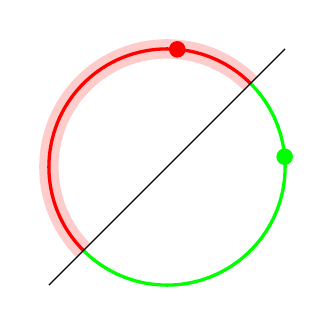
\begin{tikzpicture}
  \draw[very thick, green] (45:1.5) arc (45:-135:1.5);
  \draw[very thick, red] (45:1.5) arc (45:225:1.5);
  \draw[line width=7pt, red, opacity=0.2] (45:1.5) arc (45:225:1.5);
  \draw (1.5,1.5)--(-1.5,-1.5);
  \fill[green] (5:1.5) circle (3pt);
  \fill[red] (85:1.5) circle (3pt);
\end{tikzpicture}




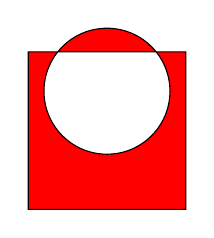
\begin{tikzpicture}
\filldraw[fill=red,even odd rule]
(0,0) rectangle (2,2) (1,1.5) circle (0.8cm);
\end{tikzpicture}


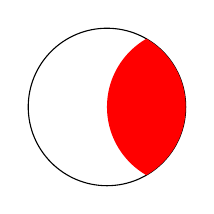
\begin{tikzpicture}
\draw[clip] (0,0) circle (1cm);
\fill[red] (1,0) circle (1cm);
\end{tikzpicture}

%
% Заливка с контуром и без
% \begin{tikzpicture}
%   \draw (0,0) circle (1pt);
% \end{tikzpicture}
% \begin{verbatim}
% \end{verbatim}

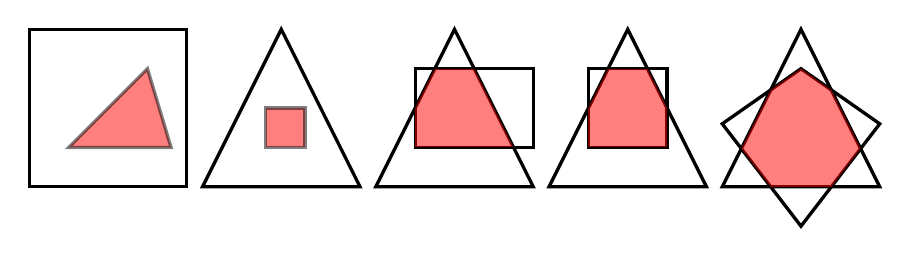
\begin{tikzpicture}
    \draw [very thick] (0,0) -- (0,2) -- (2,2) -- (2,0) -- cycle;
    \draw [fill = red, opacity = 0.5, very thick] (0.5,0.5) -- (1.5,1.5) -- (1.8,0.5) -- cycle;
    \draw [xshift=2.2cm, very thick] (0,0) -- (1,2) -- (2,0) -- cycle;
    \draw [xshift=2.2cm,fill = red, opacity = 0.5, very thick] (0.8,0.5) -- (0.8,1) -- (1.3,1) -- (1.3,0.5) -- cycle;
    \begin{scope}
        \draw [xshift=4.4cm, very thick] (0.5,0.5) -- (0.5,1.5) -- (2,1.5) -- (2,0.5) -- cycle;
        \draw [very thick,xshift=4.4cm] (0,0) -- (1,2) -- (2,0) -- cycle;
        \draw [clip,xshift=4.4cm] (0,0) -- (1,2) -- (2,0) -- cycle;
        \fill [red, opacity = 0.5, xshift=4.4cm, very thick] (0.5,0.5) -- (0.5,1.5) -- (2,1.5) -- (2,0.5) -- cycle;
    \end{scope}
     \begin{scope}
        \draw [xshift=6.6cm, very thick] (0.5,0.5) -- (0.5,1.5) -- (1.5,1.5) -- (1.5,0.5) -- cycle;
        \draw [very thick,xshift=6.6cm] (0,0) -- (1,2) -- (2,0) -- cycle;
        \draw [clip,xshift=6.6cm] (0,0) -- (1,2) -- (2,0) -- cycle;
        \fill [red, opacity = 0.5, xshift=6.6cm, very thick] (0.5,0.5) -- (0.5,1.5) -- (1.5,1.5) -- (1.5,0.5) -- cycle;
    \end{scope}
     \begin{scope}
        \draw [xshift=8.8cm, very thick] (1,-0.5) -- (0,0.8) -- (1,1.5) -- (2,0.8) -- cycle;
        \draw [very thick,xshift=8.8cm] (0,0) -- (1,2) -- (2,0) -- cycle;
        \draw [clip,xshift=8.8cm] (0,0) -- (1,2) -- (2,0) -- cycle;
        \fill [red, opacity = 0.5, xshift=8.8cm, very thick]  (1,-0.5) -- (0,0.8) -- (1,1.5) -- (2,0.8) -- cycle;
    \end{scope}
\end{tikzpicture}

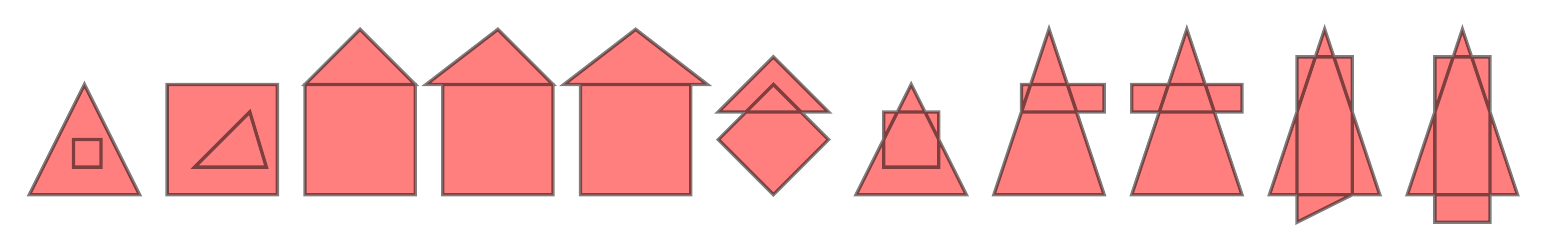
\begin{tikzpicture}[scale=0.7]
    \draw [fill = red, opacity = 0.5, very thick] (0,0) -- (1,2) -- (2,0) -- cycle
    (0.8,0.5) -- (0.8,1) -- (1.3,1) -- (1.3,0.5) -- cycle;

    \draw [xshift=2.5cm,fill = red, opacity = 0.5, very thick] (0,0) -- (0,2) -- (2,2) -- (2,0) -- cycle
     (0.5,0.5) -- (1.5,1.5) -- (1.8,0.5) -- cycle;

    \draw [xshift=5cm,fill = red, opacity = 0.5, very thick] (0,0) -- (0,2) -- (2,2) -- (2,0) -- cycle
     (0,2) -- (1,3) -- (2,2) -- cycle;

    \draw [xshift=7.5cm,fill = red, opacity = 0.5, very thick] (0,0) -- (0,2) -- (2,2) -- (2,0) -- cycle
     (-0.3,2) -- (1,3) -- (2,2) -- cycle;

    \draw [xshift=10cm,fill = red, opacity = 0.5, very thick] (0,0) -- (0,2) -- (2,2) -- (2,0) -- cycle
     (-0.3,2) -- (1,3) -- (2.3,2) -- cycle;

    \draw [xshift=12.5cm,fill = red, opacity = 0.5, very thick] (1,0) -- (0,1) -- (1,2) -- (2,1) -- cycle
    (0,1.5) -- (1,2.5) -- (2,1.5) -- cycle;

    \draw [xshift=15cm,fill = red, opacity = 0.5, very thick] (0.5,0.5) -- (0.5,1.5) -- (1.5,1.5) -- (1.5,0.5) -- cycle
    (0,0) -- (1,2) -- (2,0) -- cycle;

    \draw [xshift=17.5cm,fill = red, opacity = 0.5, very thick] (0.5,1.5) -- (0.5,2) -- (2,2) -- (2,1.5) -- cycle
     (0,0) -- (1,3) -- (2,0) -- cycle;

    \draw [xshift=20cm,fill = red, opacity = 0.5, very thick] (0,1.5) -- (0,2) -- (2,2) -- (2,1.5) -- cycle
     (0,0) -- (1,3) -- (2,0) -- cycle;

    \draw [xshift=22.5cm,fill = red, opacity = 0.5, very thick] (0.5,-0.5) -- (0.5,2.5) -- (1.5,2.5) -- (1.5,0) -- cycle
        (0,0) -- (1,3) -- (2,0) -- cycle;

    \draw [xshift=25.0cm,fill = red, opacity = 0.5, very thick] (0.5,-0.5) -- (0.5,2.5) -- (1.5,2.5) -- (1.5,-0.5) -- cycle
     (0,0) -- (1,3) -- (2,0) -- cycle;
\end{tikzpicture}



%\ЛичныйКондуит{0mm}{6mm}
\end{document}



